%Title of section
\section{研究动机}

\subsection{主要目标}

\begin{frame}
\frametitle{研究动机}
\framesubtitle{主要目标}
\begin{block}{解决CaaS模式下云数据中心的能耗优化问题}
    \begin{itemize}
        \item 负载监控机制:负载与能耗紧密相关
        \begin{itemize}
            \item 实时性
            \item 准确性
            \item 易扩展性
        \end{itemize}
        \item 基于负载状态容器调度策略
        \begin{itemize}
            \item 保证云服务QoS(Quality of Service)
            \item 降低整体能耗
        \end{itemize}
    \end{itemize}
\end{block}
\end{frame}

\subsection{负载监控}

\begin{frame}
\frametitle{研究动机}
\framesubtitle{负载监控}
容器负载监控机制对云数据中心\textbf{\alert{资源配置和调度决策}}有较大影响

\begin{block}{负载监控机制}
\begin{itemize}
    \item<1-> 基于负载采集程序:负载变化频繁、异构网络环境导致滞后性
    \item<2-> 负载预测模型:主动进行资源配置和容器调度
\end{itemize}
\end{block}
\begin{figure}[htb]
\centering
    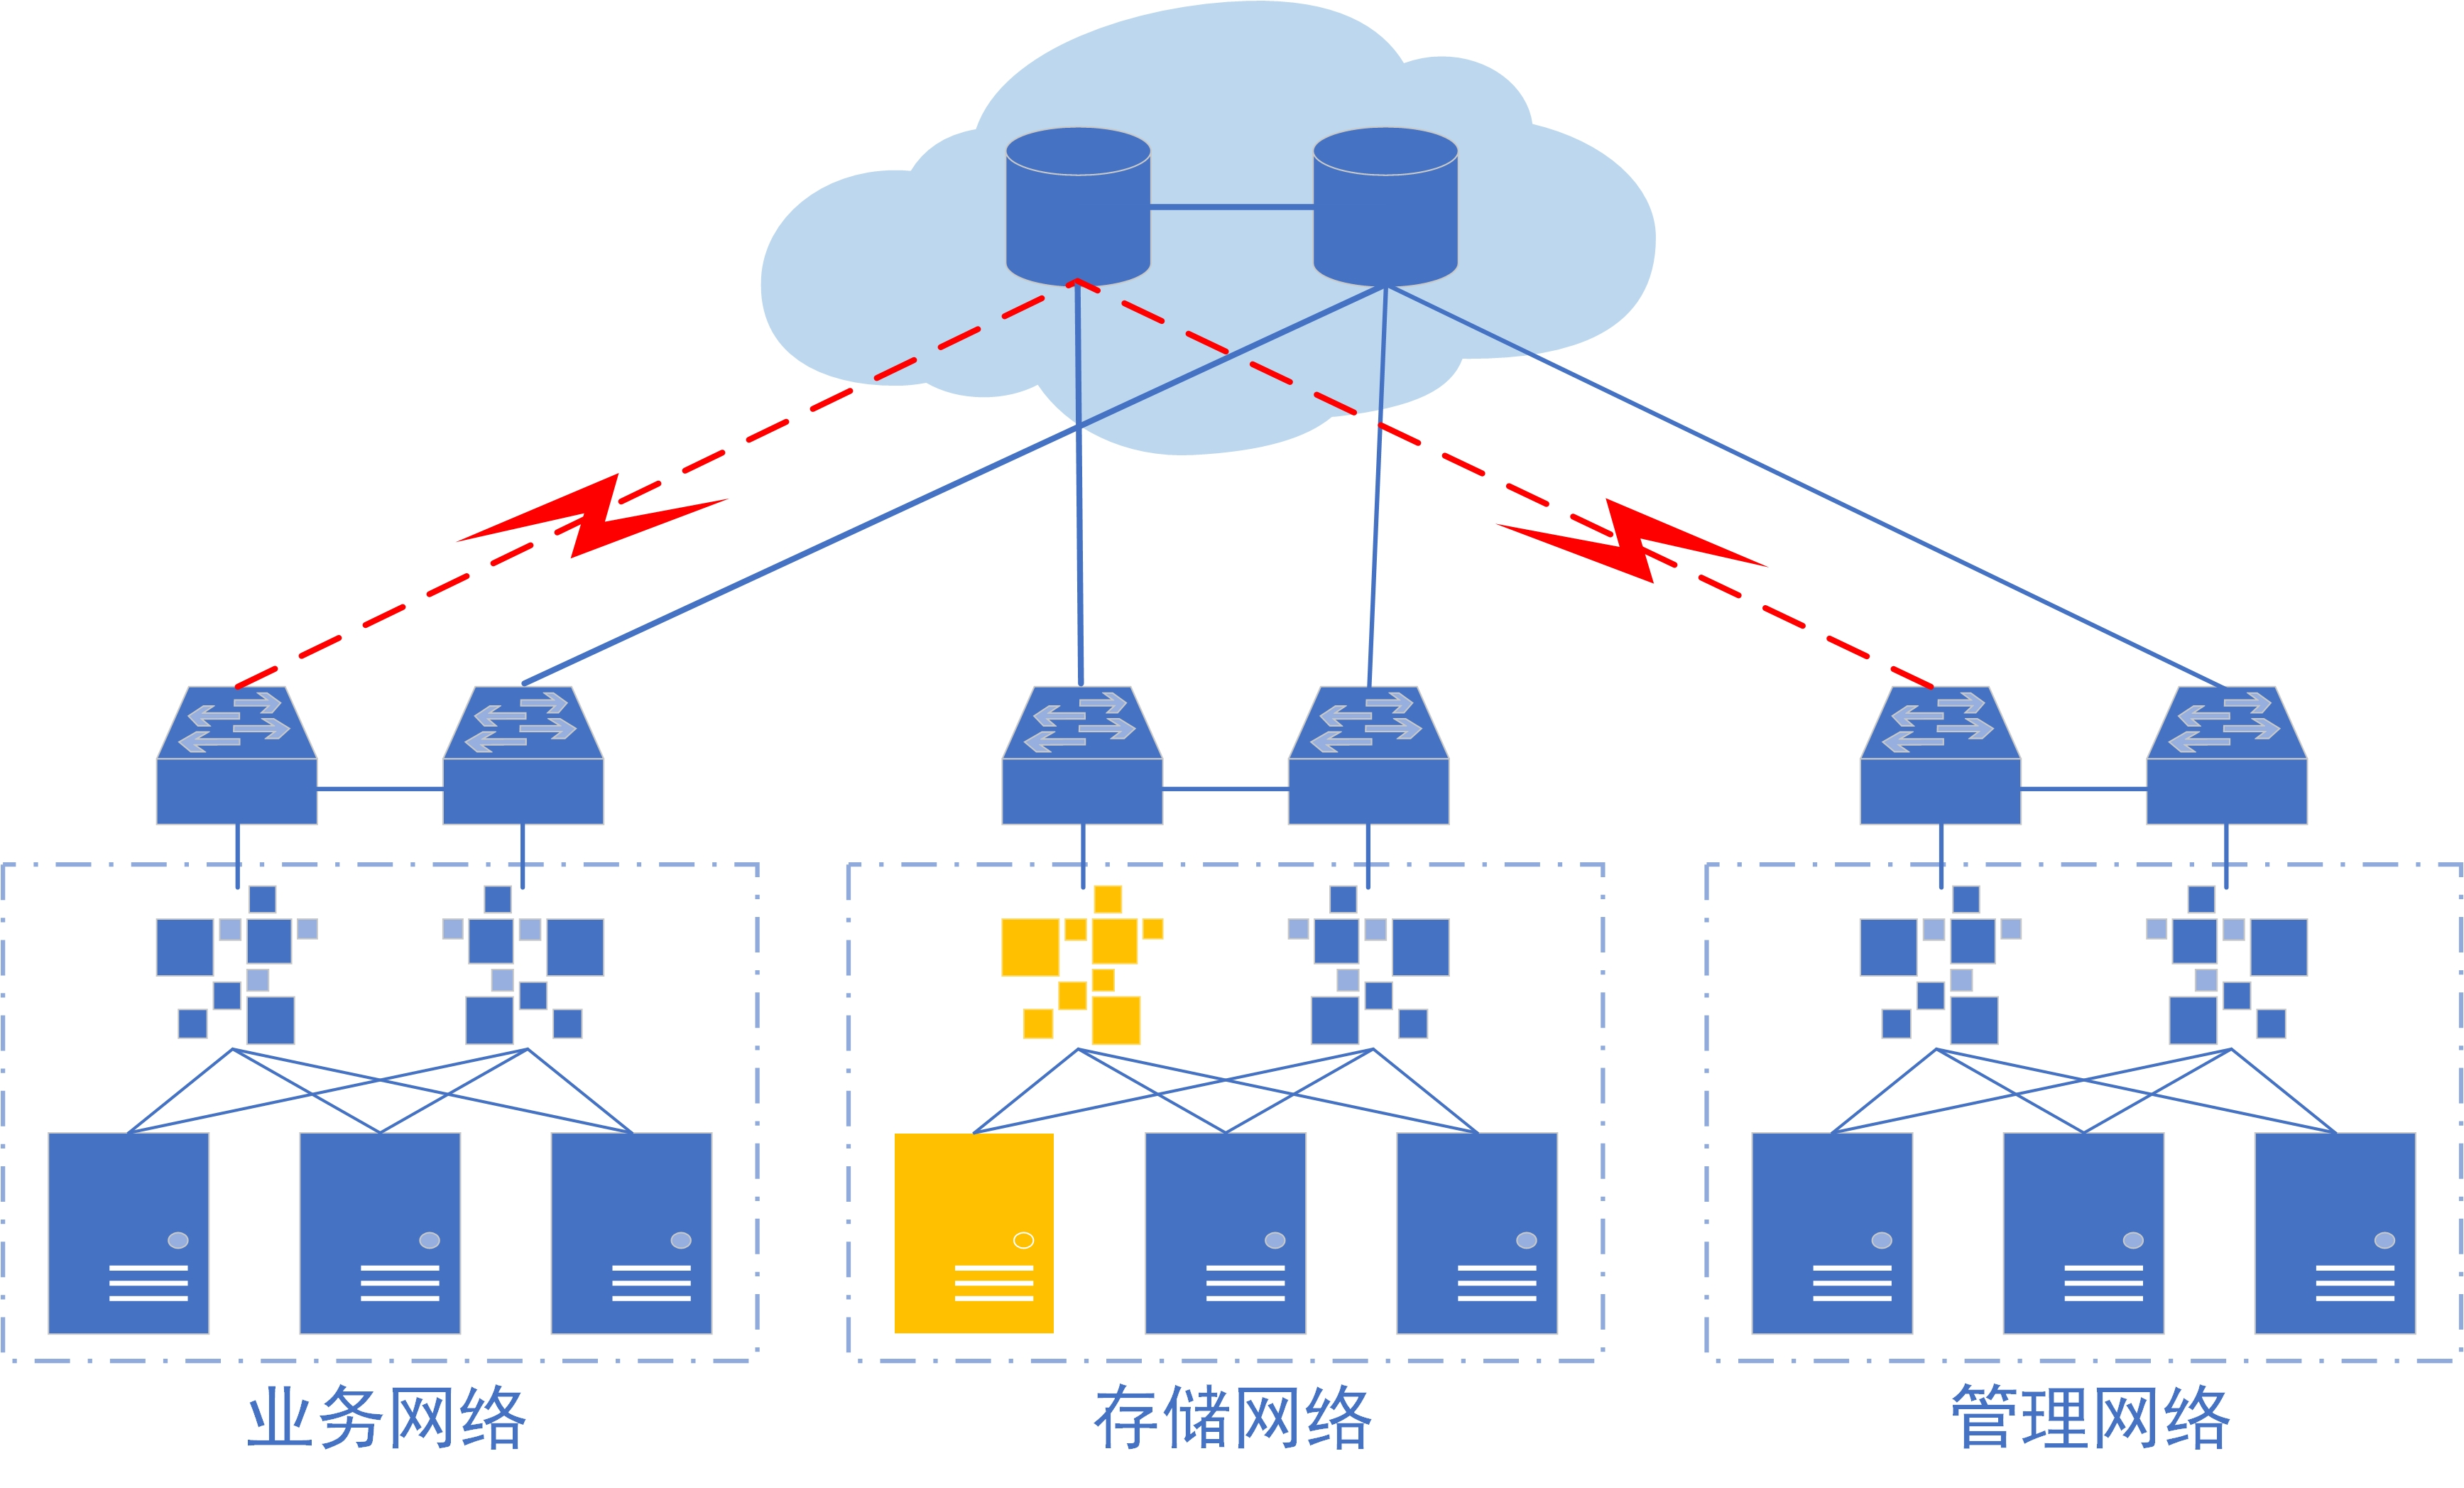
\includegraphics[scale=0.41]{figures/fig3_mmn.jpg}
    \caption{基于负载采集程序的监控网络}
    \label{fig:fig3}
\end{figure}
\end{frame}

\begin{frame}
\frametitle{研究动机}
\framesubtitle{负载监控}
\begin{block}{负载预测模型}
\begin{itemize}
    \item<1-1> 单值预测模型:预测特定值
    \begin{itemize}
        \item<1-1> \textbf{误差敏感} $\Rightarrow$ \textbf{决策失效}
        \item<1-1> \textbf{鲁棒性差} $\Rightarrow$ \textbf{决策过度}
    \end{itemize}
    \item<2-2> 区间预测模型\textsuperscript{$\star$}:预测取值区间(置信度$\alpha=0.9$)
\end{itemize}
\end{block}

\vspace*{-0.7cm}
\visible<1>{
\begin{columns}
\begin{column}{0.6\textwidth}
    \centering
    \begin{table}[hftb]
    \centering
    \resizebox{\textwidth}{!}{%
        \begin{tabular}{ccl}
            \toprule
            \textbf{类型} & \textbf{模型名称} & \textbf{简述}\\
            \midrule
            \multirow{4}{*}{统计学模型} & ARIMA & 差分自回归移动平均\\
            ~ & Kalman滤波 & 基于递推演进和观测值对预测结果进行演进\\
            ~ & 排队论模型 & 基于在线作业请求和系统阻塞情况进行预测\\
            ~ & 灰色模型 & 模型新陈代谢过程,进行中长期预测\\
            \midrule
            \multirow{4}{*}{机器学习模型} & RNN & 递归神经网络预测\\
            ~ & BPNN & 原始信息前向传播,误差信息后向传播\\
            ~ & LSTM & 长短期记忆网络\\
            ~ & 混合模型 & 基于c-means聚类和模糊(Fuzzy)神经网络\\
            \bottomrule
        \end{tabular}
    }
    \caption{单值预测模型}
    \end{table}
\end{column}
\begin{column}{0.3\textwidth}
\centering
\begin{figure}[htb]
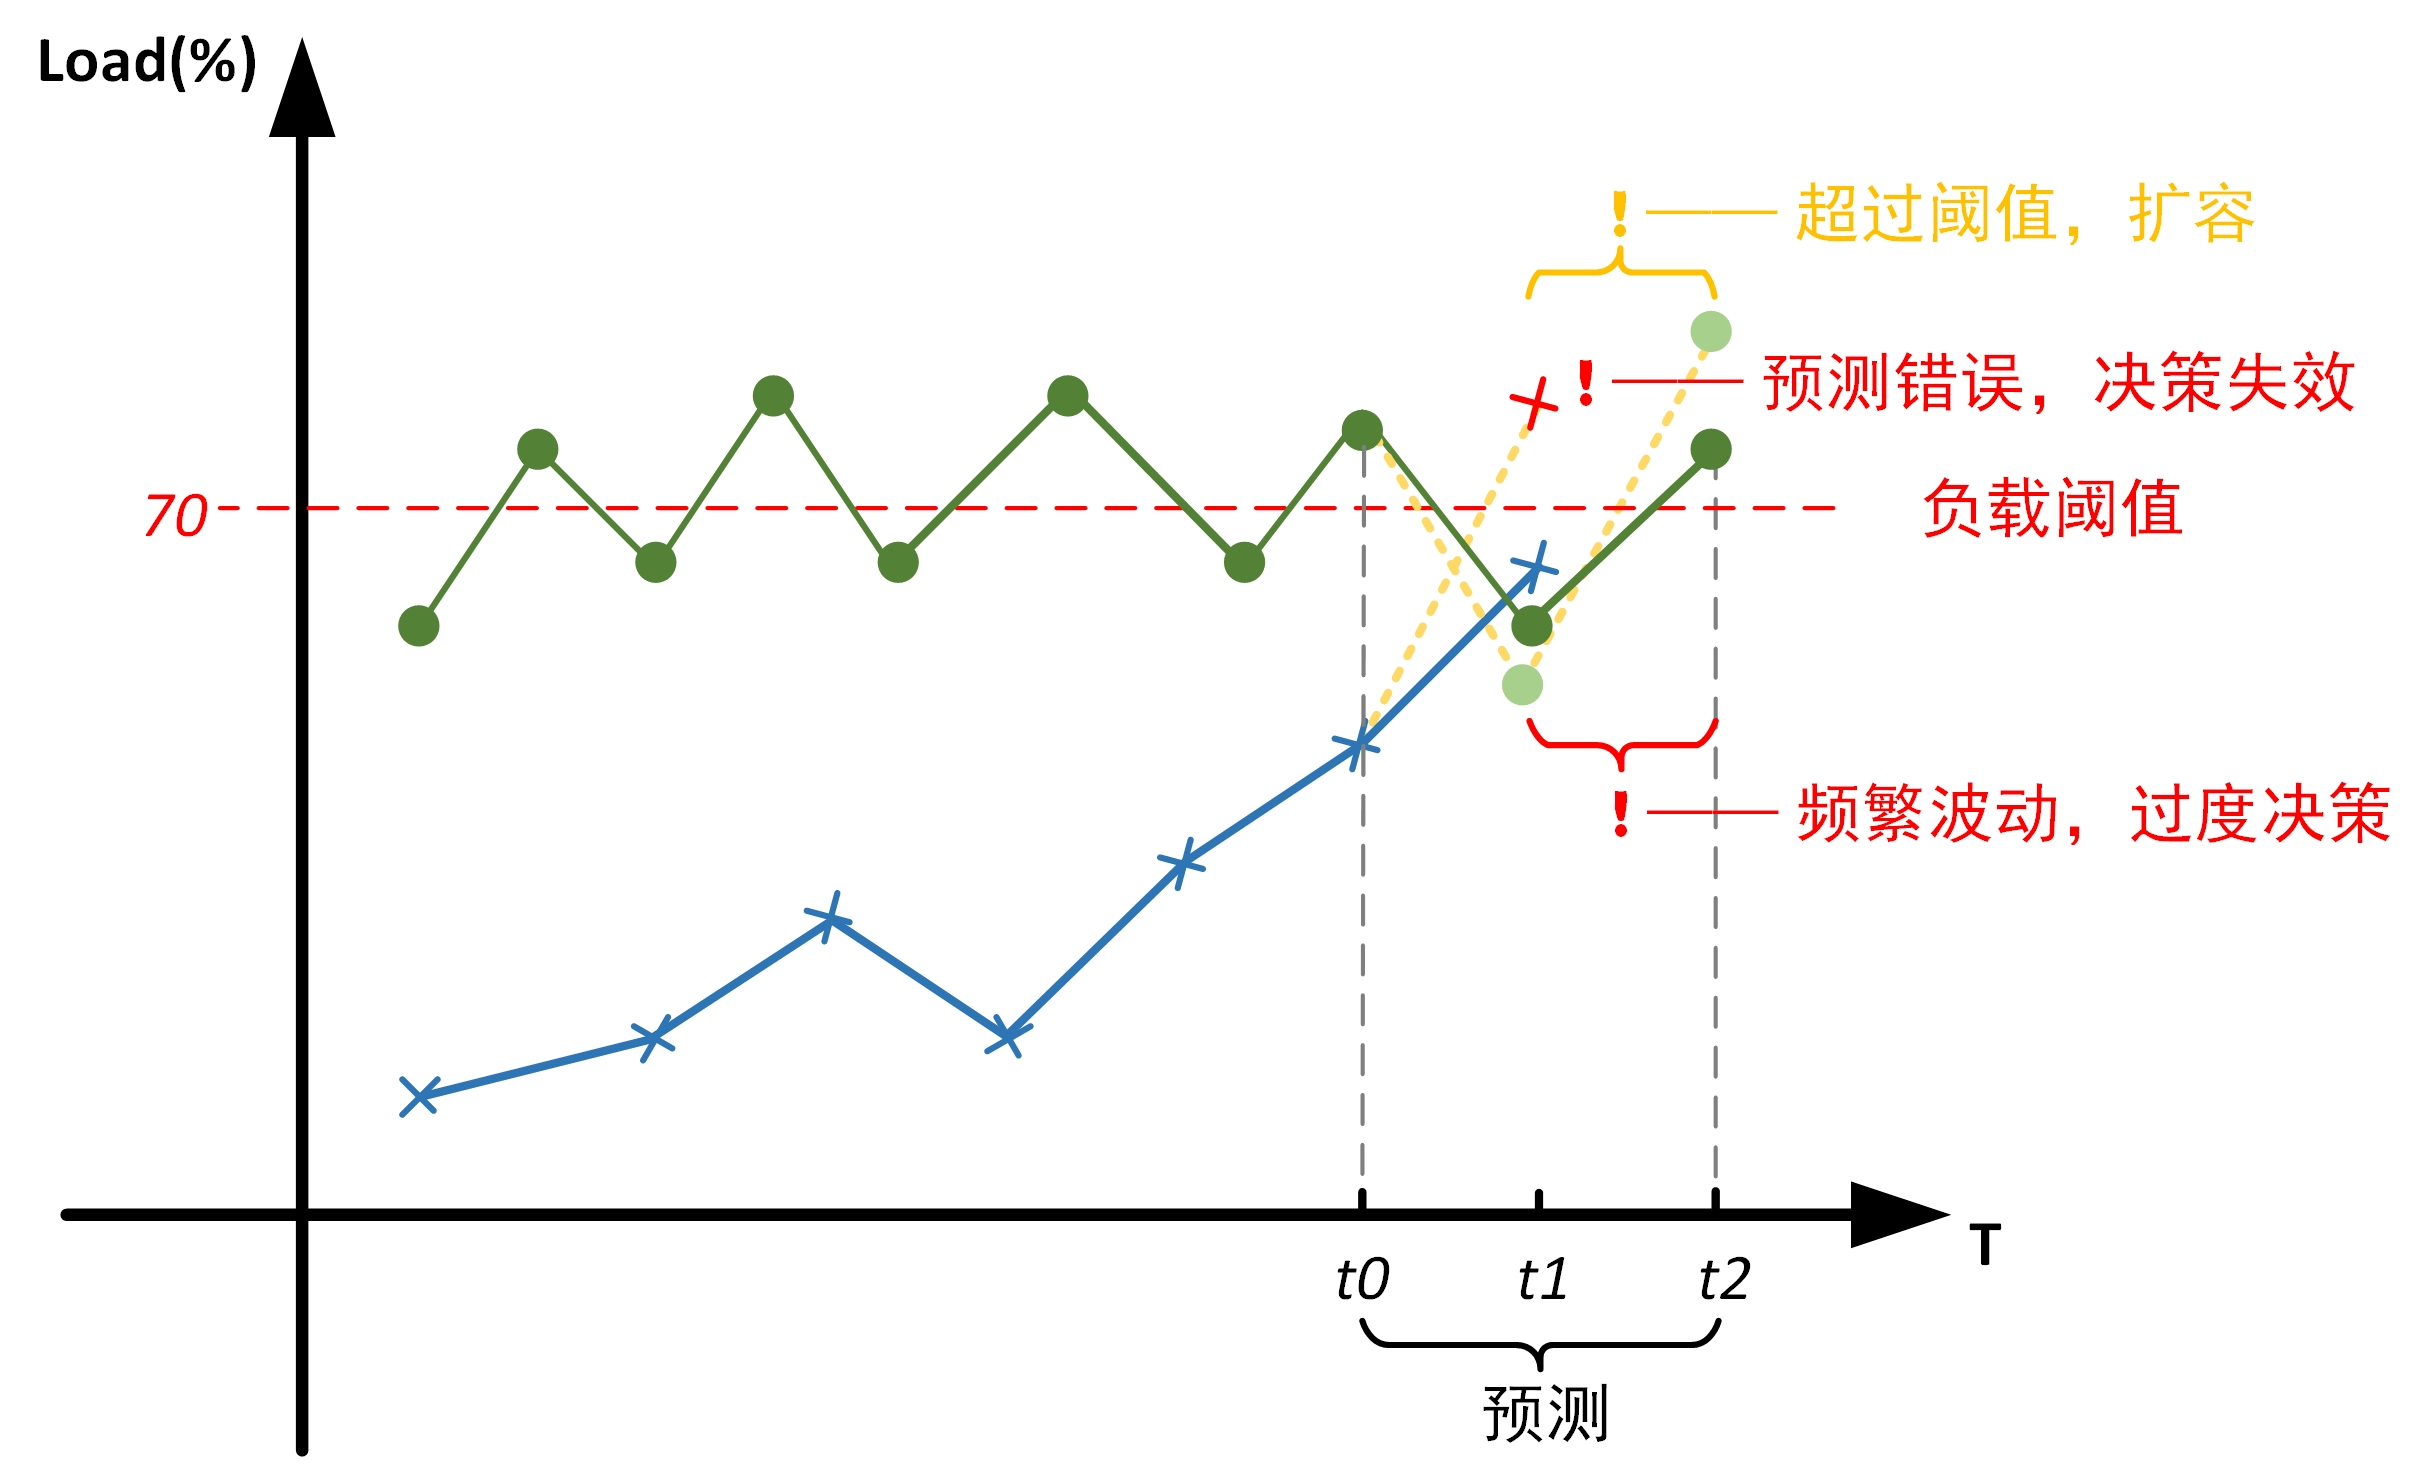
\includegraphics[scale=0.4]{figures/fig4_single_model.jpg}
\caption{单值预测模型}
\end{figure}
\end{column}
\end{columns}
}
\vspace*{-4.54cm}
\visible<2>{
\begin{columns}
\begin{column}{0.6\textwidth}
    \begin{table}[hftb]
    \centering
    \resizebox{\textwidth}{!}{%
        \begin{tabular}{ccl}
            \toprule
            \textbf{类型} & \textbf{模型名称} & \textbf{简述}\\
            \midrule
            概率论模型 & 贝叶斯模型 & 根据样本分布假设和统计学特征扩展区间\\
            \midrule
            \multirow{4}{*}{机器学习模型} & 线性回归 & \multirow{4}{*}{先拟合单值再根据分布假设构建区间}\\
            ~ & SVM & \\
            ~ & CART & \\
            ~ & 随机森林 & \\
            \bottomrule
        \end{tabular}
    }
    \caption{区间预测模型}
    \end{table}
\end{column}
\begin{column}{0.3\textwidth}
\end{column}
\end{columns}
}
\end{frame}

\subsection{容器调度}

\begin{frame}
\frametitle{研究动机}
\framesubtitle{容器调度}
\end{frame}